\section{Towards Generic Parallel Programming}\label{chap:background}

A programming model is an abstract representation of a computer. It defines a paradigm and a programming language. The programming language is used by the programmer to write source code, a human-readable textual representation of instructions and data. Source code is a sequential listing of statements evaluated from the top to bottom, one line at a time. While such ordering seems natural to describe an algorithm as it corresponds to sequential processing (both, reading code and progressing the program counter follow a time line), it does not include the notion of concurrency.

Parallel programming models add the notion of concurrency to a sequence of instruction of a program. This is commonly achieved either by adding semantic value to the base programming language, often referred to as programming with \emph{pragma} annotations, through library calls or new languages. All three approaches are conceptually suitable to represent programming paradigms such as tasking, parallel patterns and others. Well known representatives are the OpenMP programming model~\cite{CITEOPENMP} or threading libraries respectively. In general, it is up to the parallel programming model to expose language constructs or library interfaces (APIs) such that they are convenient to the programmer and capture enough semantic information to allow the programming model to map the program execution to the parallel computer hardware efficiently and correctly. Questions of which semantic information is needed, what paradigm to present and by what syntactical means span a design space worth taking a closer look at. Figure~\ref{figSemCapture} shows the three areas that constitute a parallel programming model and its design. We call it the semantic capture.

\begin{figure}[h]
\begin{Verbatim}[frame=leftline]
Semantic information
Paradigm 
Language
\end{Verbatim}
\caption{Semantic capture - a triplet of language, paradigm and semantic information defined by a parallel programming model allow the programmer to express concurrency and the compiler and runtime system to understand and run applications on a parallel machine.}
\label{figSemCapture}
\end{figure}

Semantic information provided by the programmer to the parallel programming model can be grouped into information to express intent and properties. They address the question of \emph{what}, \emph{where} and \emph{how}, which, in the context of parallel programming, corresponds to defining which code portion to parallelize, where to run and access and how to run that parallel code. Synchronization primitives may be considered as part of the what and information on the execution properties such as data placement or memory access type as the how. Semantics are expressed following a paradigm and a programming language.

The parallel programming paradigm is an abstract ~\emph{representation} with the purpose of facilitating the programmer's understanding of programming rules and program behavior. Which programming paradigm to chose depends on several considerations. Parallel-patterns allow to express concurrency for commonly occurring programming patterns such as loop constructs. Tasking is a paradigm that support the expression of concurrent loops as well as irregular algorithms. Distributed and correctness-oriented programming models may implement actor-based programming. In this programming model, each unit of execution represent an actor who communicates over predefined communication interfaces. This paradigm eliminates accesses to shared state and align well with message passing programming (MPI). The execution model and memory model of a programming model defines behavior. That is, it defines the relationship between abstract concepts and program behavior on the given architecture.

Lastly, a language defines the syntax of the parallel semantic. Declarative languages add semantic information to the base language through pragma annotations while imperative languages rely on programming interfaces to capture information. Their semantic is defined in the API specification. Figures~\ref{figOMPLike} and~\ref{figKokkosLike} show examples of two sample applications using the aforementioned parallel programming language types. While both programming models implement the same programming paradigm (parallel patterns), Figures~\ref{figOMPLike} extends the base programming language through pragma annotations. Both, pragma annotations and an API call as shown in Figure~\ref{figKokkosLike} have a similar semantic of describing a parallel loop construct. It is up to the programming model specification to define the execution and memory model in both cases. 

Both examples provide the semantic information on what to parallelize, however, they do not provide information on how to map the parallel execution on modern parallel architectures. In order to define what further information is needed for a generic support on concurrency on modern computer architectures, it is important to define an abstract machine model first.

\begin{figure}
\begin{Verbatim}[frame=leftline]
# pragma model parallel for
for ( size_t i = 0; i < N; ++i) {
 /* loop body */
}
\end{Verbatim}
\caption{Declarative parallel programming provides uses pragma annotations to capture semantic information.}
\label{figOMPLike}
\end{figure}

\begin{figure}
\begin{Verbatim}[frame=leftline]
model::parallel_for (N, [=] ( const size_t i) {
  /* loop body */
});
\end{Verbatim}
\caption{Imperative parallel programming uses a base language and relies on programming interfaces to capture information and a documentation that describe their semantics.}
\label{figKokkosLike}
\end{figure}

\section{The Kokkos Abstract Machine Model}\label{chap:kokkosMM}

The Kokkos machine model defines abstractions that represent hardware capabilities for processing and data access. The Kokkos parallel programming model exposes these abstractions to the programmer through C++ and the Kokkos API. By abstracting from physical hardware, the machine model ensures that applications written in programming models targeting this machine model are generic and performance-portable on current and future hardware. The Kokkos parallel programming model is one particular instance of a programming model that builds on top of that machine model. We would like to point out that it is this conceptual differentiation that allows scenarios where the underlying machine model is instantiated in other languages beyond C++, yet the algorithmic specification as well as performance characteristic and portability remain the same. 

The Kokkos abstract machine model targets a design of a future shared-memory computing architectures. The design is shown in Figure~\ref{fig:execspace}. It is characterized by multiple latency-optimized execution units and off-die bandwidth-optimized accelerators. Both compute device types have disjoint memory address spaces and unique performance properties. In such an architecture,   execution units might be grouped into larger units with multiple levels of achievable parallelism with different memory access characteristics and coherence properties of caches. In order to ensure performance portability on such a wide range of configurations, an abstraction of the compute engines and available memories are required. For this purpose we introduce \emph{spaces}.

An instance of an \emph{execution space} is a specific instantiation of an execution space to which a programmer can target parallel work. For example, an execution space can be used to describe a multi-core processor. In this case, the execution space contains several homogeneous cores organized into arbitrary logical groups. In a parallel programming model that implements this machine model, an instance of such an execution space would be made available to the programmer to run kernels. Adding more logical groups or accelerators simply increases the number of available execution spaces to the programmer.

Memory and memory types are exposed through \emph{memory spaces}. Each memory space provides a finite storage capacity at which data structures can be allocated and accessed. Different memory space types have different characteristics with respect to accessibility from execution spaces and performance. 

An instance of a memory space provides a concrete method for the application programmer to request data storage allocations. Following the architecture as discussed earlier, the multi-core processor may contain multiple memory spaces that abstract on-package memory, slower DRAM and non-volatile memories. Accelerators can provide an additional memory space through its local on-package memory. The programmer is free to decide where each data structure is allocated by requesting the corresponding memory space by instantiating the according memory space. Kokkos provides the appropriate abstraction of memory allocation and data management. We believe that an abstract representation of execution- and memory devices is a key property towards performance-portable parallel programming.

How a machine model is exposed to the programmer and what are the design considerations towards defining an appropriate semantic capture are discussed in the next section.

%Ang, J.A., et. al., Abstract Machine Models and Proxy Architectures for Exascale Computing, 2014, Sandia National Laboratories and Lawrence Berkeley National Laboratory, DOE Computer Architecture Laboratories Project


\begin{figure}
\begin{subfigure}[b]{0.45\textwidth}
\centering
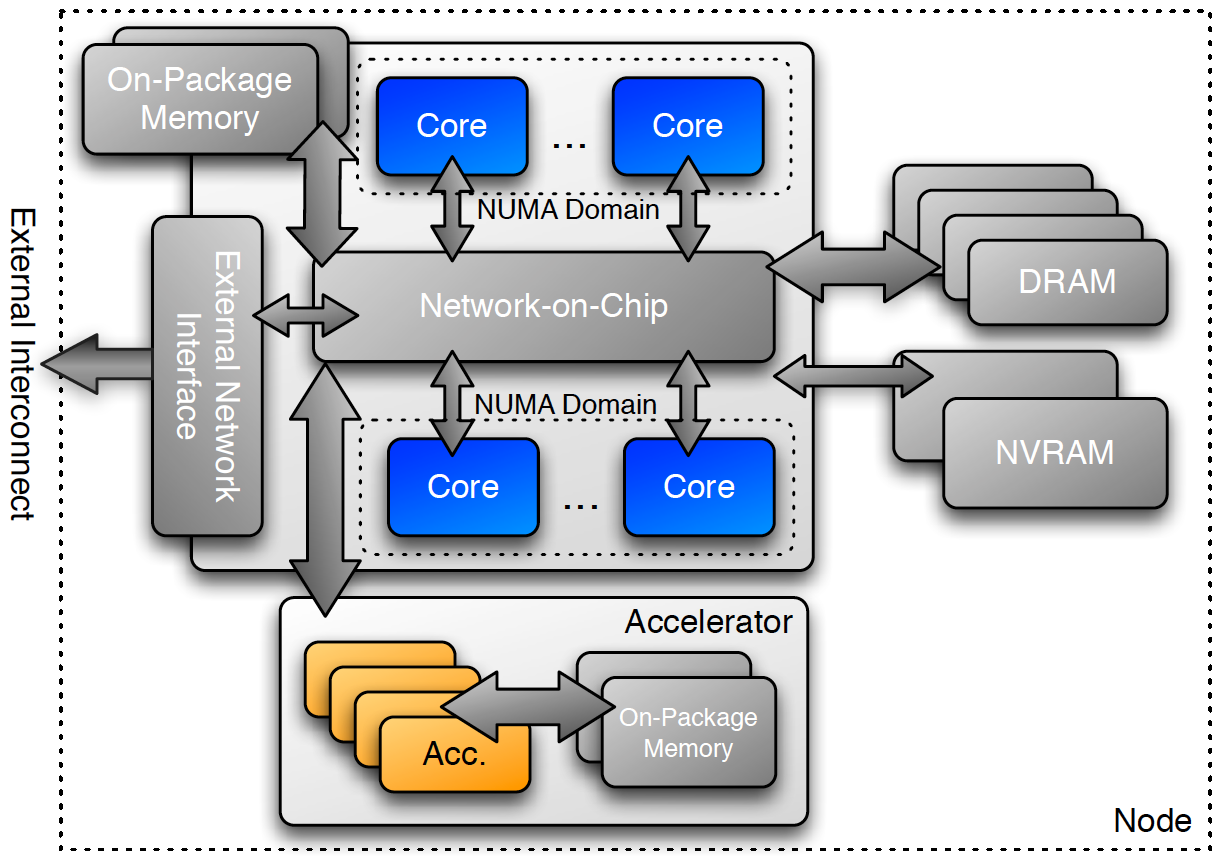
\includegraphics[width=\textwidth]{img/ExecSpaces.png}
\caption{Execution space is an instantiation of a space that represents a processing device to which the programmer can target parallel code.}
\label{fig:execspace}
\end{subfigure}%
\hfill \break
\begin{subfigure}[b]{0.45\textwidth}

\centering
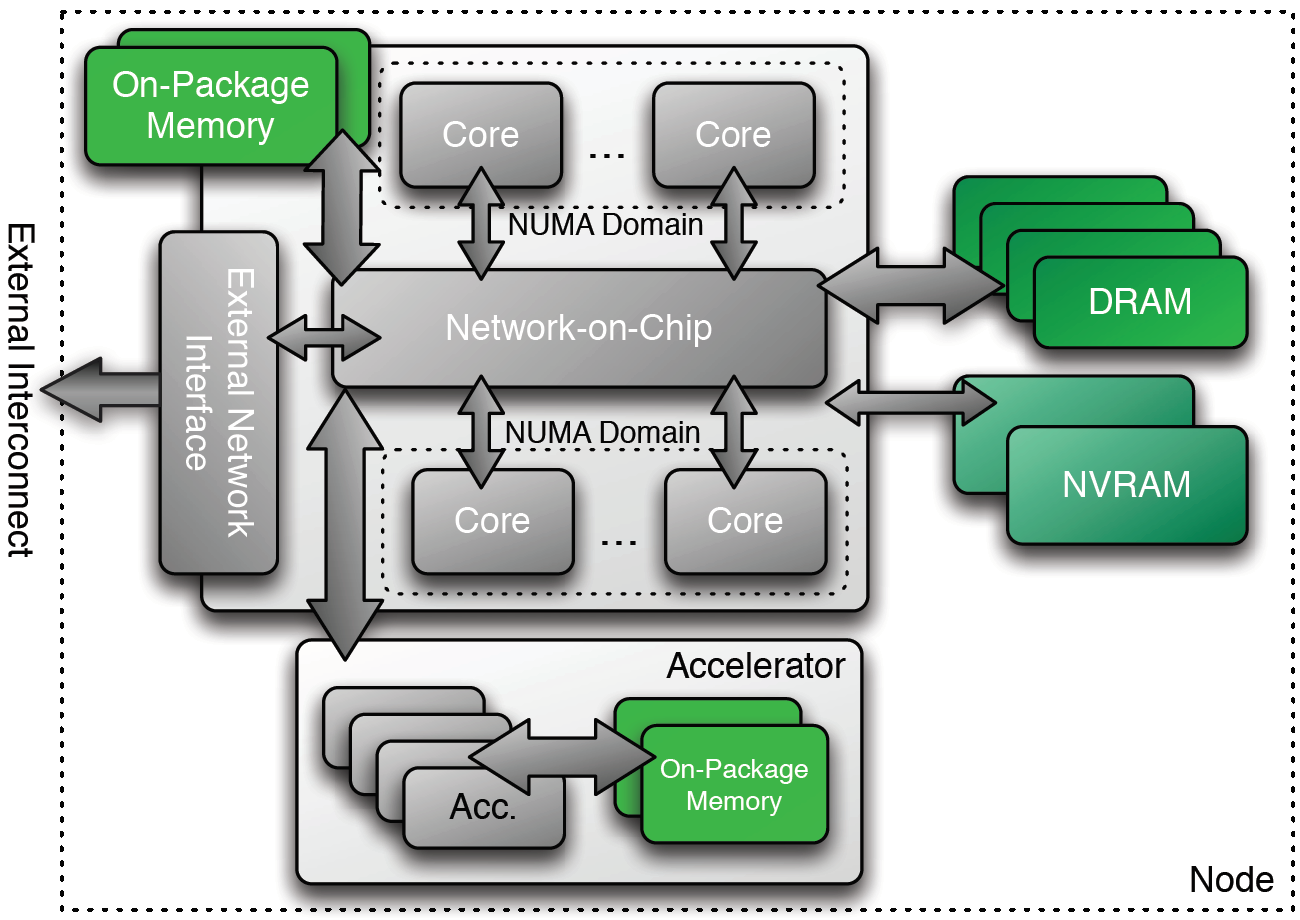
\includegraphics[width=\textwidth]{img/MemSpaces.png}
\caption{A memory space is an instantiation of a space that represents a memory location on which the programmer can allocate data.}
\label{fig:memspace}
\end{subfigure}%
\caption{Spaces represent conceptual building blocks of the abstract machine model in Kokkos.}
\label{fig:spaces}
\end{figure}

\section{The Kokkos Programming Model}\label{chap:kokkosPM}
%====================
The Kokkos programming model specifies a language, programming paradigm and an API. The API exposes the abstract machine model to the developer and defines a set of pattens and types that capture intents and properties of execution. This completes the semantic capture, discussed in Chapter~\ref{chap:background}, We detail all three components as follows.

Kokkos defines a pure interface for C++ and uses C++ as the base programming language. This has multiple reasons. It is our experience that application developers of scientific and high-performance computing applications at Sandia National Laboratories express the demand for C++ and a generic parallel programming model to support their codes. Following their estimates, porting efforts towards adapting to vendors, programming models, APIs and software releases represents a burden worth addressing. Further, the possibility to maintain pure C++ codes is appealing from the code development and debugging perspective. 
Lastly, from the programming model perspective, C++ offers template metaprogramming which is well suited to implement generic APIs and libraries. In this case, class specialization and templating allow for compile-type generated types and optimizations for a given hardware architecture. It is worth to mention that Kokkos avoids the use of pragma annotations for the sake of treating concurrency as a first-class concept in C++.

Using the programming language, a parallel programming paradigm can be applied to simplify the process of thought. Kokkos supports the parallel patterns and task paradigms. Parallel patters covers \emph{for}, \emph{ scan} and \emph{reduction}. This allows the expression of concurrency over iterative, for-loop computable algorithms. To cover the class of while-loop computable algorithms (irregular algorithms), Kokkos implements the tasking paradigm. Tasks encapsulate work into units that may be executed in parallel to other tasks or sections of the program. Equipped with a language and set of paradigms, a particular set of abstractions can be defined to expose the abstract machine model and captures the intent of the programmer.


\subsection{Kokkos Abstractions}

To capture semantic information, that is the~\emph{What}, the ~\emph{Where} and the ~\emph{How}, Kokkos introduces six abstractions: \emph{execution spaces}, \emph{execution patterns}, \emph{execution policies}, \emph{memory spaces}, \emph{memory layout} and \emph{memory traits}. These abstractions specify semantic information that enable to capture the programmer's intent and the runtime to efficiently map the program to any underlying hardware architecture. We list them as follows:
\begin{itemize}
	\item  An execution space is a place where code can be executed. On current hardware architectures this correspond to accelerators and CPUs and can include any compute device in the future. This abstraction supports remote compute devices in distributed memory scenarios as remote execution spaces.
	\item Execution patterns expose the parallel programming paradigm. Supported patterns are \emph{parallel\_for} loop that executes the loop body in any order a specified amount of times, the \emph{parallel\_reduce} which combines a parallel\_for with a reduction operation, \emph{parallel\_scan} which combines a parallel\_for operation with a prefix or postfix scan, and \emph{task} which executes a single function potentially in parallel in respect to other tasks or code sections. 
	\item Execution policy shape the iteration space of a loop pattern. A simple execution policy is a range policy. It specifies that the loop body is executed once for each element in a range.
	\item Memory spaces are the places where data resides. They specify physical locations of data as well as access characteristics. Different physical locations correspond to different device types such as high bandwidth memories, on-die scratch memories or non-volatile bulk storage. Different logical memory spaces allow for concepts such as UVM memory in the CUDA programming model, which is accessible from the host and the CUDA accelerator. Memory spaces, similarly to execution spaces, conceptually support remote memory locations in distributed-memory scenarios. Furthermore, they encapsulate functionality such as consistency control and persistence scopes.
	\item Layouts express the mapping from loop indices to address offsets. By adopting appropriate layouts for memory structures, an application can optimize data access patterns in a given algorithm. If an implementation provides polymorphic layouts (i.e. a data structure can be instantiated at compile or runtime with different layouts), architecture-dependent optimizations can be performed.
	\item Memory traits specify how a data structure is accessed. Traits express usage scenarios such as atomic access, random access and streaming loads or stores. This allows the programming model to  optimize load and store operations.
\end{itemize}


\begin{figure}[h]
\begin{Verbatim}[frame=leftline]
Semantic information: Patterns (intent), Spaces, Layouts, 
Policies and Traits
Paradigm: Parallel patterns and tasking
Language: C++
\end{Verbatim}
\caption{Semantic capture defining the Kokkos programming model.}
\label{fig:SemCaptureKokkos}
\end{figure}

Expressing concurrency with patterns and abstractions allows the compiler to generate optimized transformations. Further, a runtime library to map the execution to the parallel hardware. In the case of parallel patterns, the execution is unspecified and only promise deterministic results for the reduction and scan operations. This gives the freedom to the underlying abstraction layers to implement different mapping patterns on different hardware such as assignment of iterations to threads or vector lanes. We believe that these abstraction and their descriptive semantic represent key programming primitives and the way forward for native language support for parallel programming.
Figure~\ref{fig:SemCaptureKokkos} shows the semantic capture definition of the Kokkos programming model. 
Figure~\ref{fig:stack} shows abstraction layers in Kokkos and its fit in a parallel programming landscape.
The next section shows an example application written in Kokkos and provides an insight into the runtime library. For the interested reader, the complete programming model specification can be accessed on-line\cite{pub:KOKKOS}.

\begin{figure}
\begin{Verbatim}[frame=leftline]
template <class ExecPolicy, class FunctorType>
Kokkos::parallel_for(
    const std::string& name, 
    const ExecPolicy& policy, 
    const FunctorType& functor);
\end{Verbatim}
\caption{The Kokkos parallel for loop class shows how template metaprogramming allows to specialize types. Its descriptive semantic offers the freedom to optimize execution on modern architectures with multiple degrees of concurrency where an Execution policy shapes the iteration space accordingly.}
\label{fig:parallelForKokkos}
\end{figure}

%\begin{center}
%\begin{tabular}{ |c|c|c| } 
% \hline
% cell1 & cell2 & cell3 \\ 
% cell4 & cell5 & cell6 \\ 
% cell7 & cell8 & cell9 \\ 
% \hline
%\end{tabular}
%\end{center}

%\begin{figure}
%\begin{Verbatim}[frame=leftline]
%double f(){
% typedef Kokkos::Cuda ES;
% typedef Kokkos::CudaSpace MS;
% typedef Kokkos::LayoutLeft LL;
% typedef Kokkos::RangePolicy<ES> Range_policy;
% typedef Kokkos::View<double*, LL, MS> V
% V A( "A", N);
% V::HostMirror h_A = Kokkos::create_mirror_view( A );
% for ( int i = 0; i < N; ++i ) //Initialize on host
%   h_A( i ) = 1;
% Kokkos::deep_copy( A, h_A );
% double result = 0;
% Kokkos::parallel_reduce( "yAx", range_policy( 0, N ), 
%  KOKKOS_LAMBDA ( int i, double &update ) {
%   update += A( i );
% }, result );
% return result;
%}
%\end{Verbatim}
%\caption{Declarative parallel programming provides uses pragma annotations to capture semantic information.}
%\label{figOMPLike}
%\end{figure}


\begin{figure}
\centerline{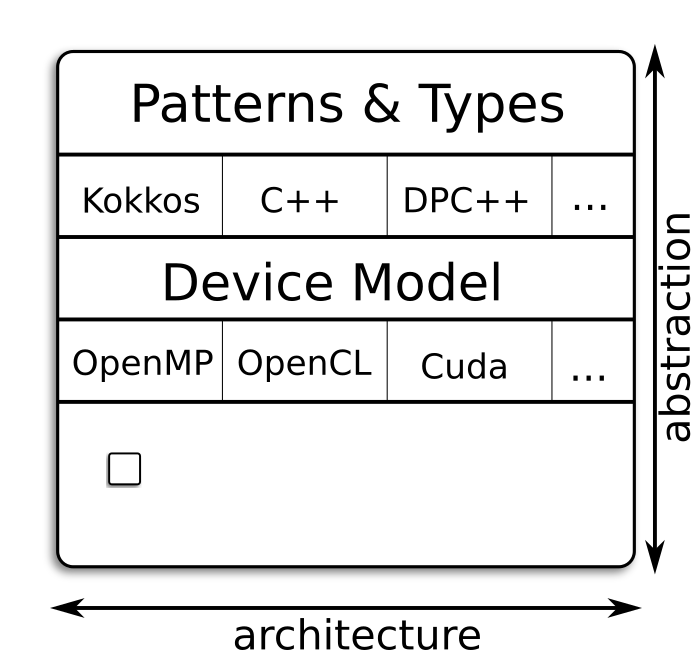
\includegraphics[width=0.3\textwidth]{img/Stack.png}}
\caption{Landscape}
\label{fig:stack}
\end{figure}


\subsection{Back-end Support}\label{chap:kokkosBackend}


The important consideration here is that the method of compiling code for different execution spaces and the dispatch of kernels to instances is abstracted by the Kokkos model. This unburdens application programmers from writing algorithms in hardware specific languages.


\begin{figure}
\centerline{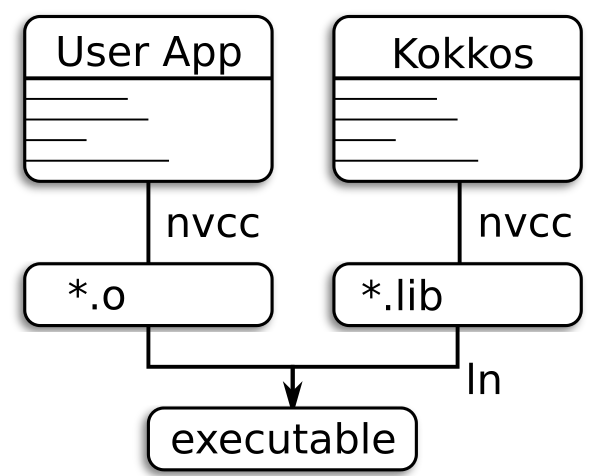
\includegraphics[width=0.3\textwidth]{img/Build.png}}
\caption{Building workflow}
\label{fig}
\end{figure}

